\chapter{Implementação e resultados}
\label{cap:implementacaoresultados}

Neste capítulo será detalhado a implementação, com a configuração do \ac{OS}, do ambiente virtualizado e das ferramentas que irão compôr o
\textit{cluster} de alta disponibilidade. Posteriormente, serão efetuados testes e medições de resultados.

Nas próximas seções será demonstrado a configuração das ferramentas do ambiente de alta disponibilidade, do ambiente de virtualização e 
também do sistema operacional.

Descrever o que nao deu certo no projeto com o ganeti??

\section{Topologia}

A estrutura física adotada está representada na Figura \ref{fig:projeto_fisico}.

\begin{figure}[h!]
 \centering
 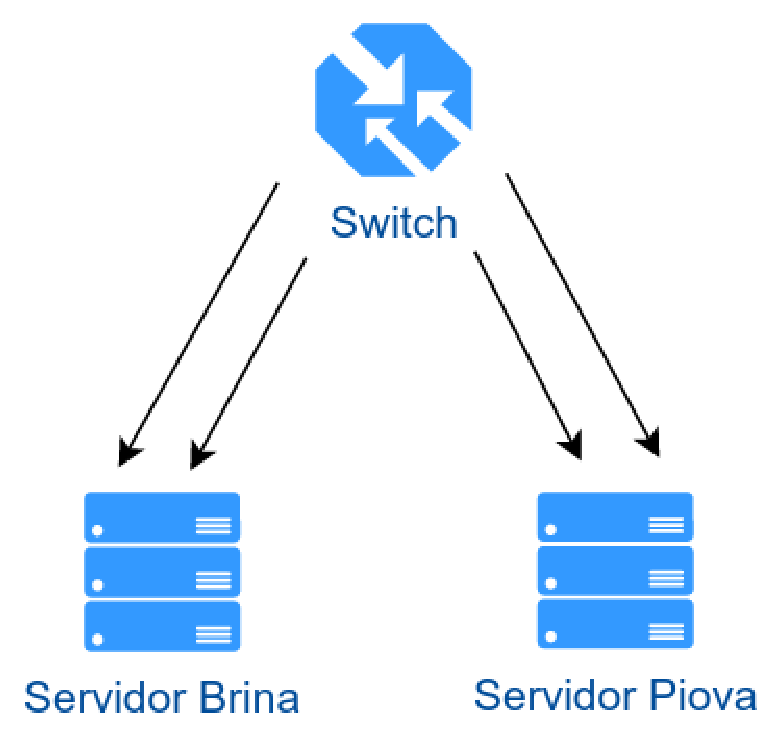
\includegraphics[width=180px]{img/projeto_fisico.eps}
 \caption{Estrutura física.}
 \label{fig:projeto_fisico}
\end{figure}

Pode-se observar os dois servidores ligados a um \textit{switch} através de dois cabos UTP cada servidor ...

Na Figura \ref{fig:servidores_brina_piova} tem-se a imagem dos servidores, o primeiro no topo da imagem, \textit{Brina} 
(\textit{Dell PowerEdge 2950}), e o servidor mais abaixo, \textit{Piova} (\textit{Dell PowerEdge R410}).

\begin{figure}[h!]
 \centering
 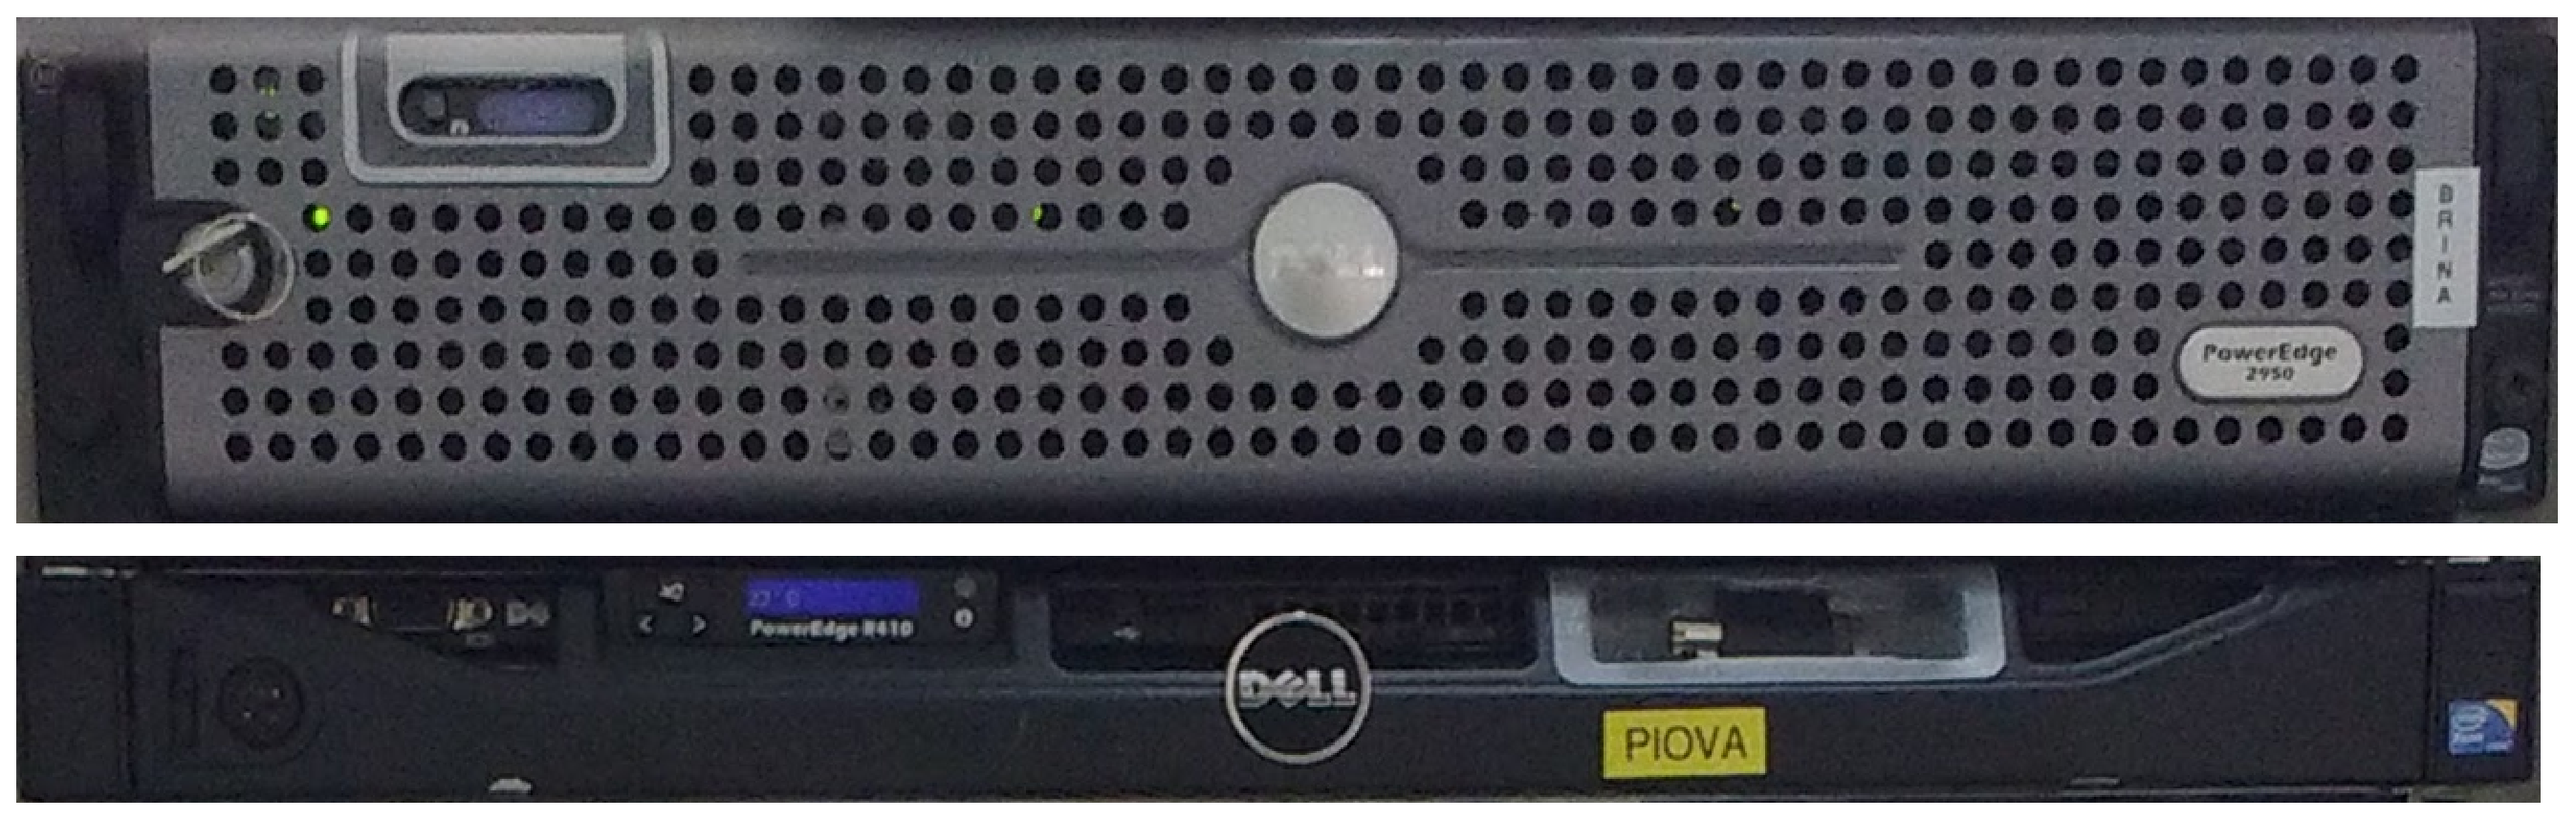
\includegraphics[width=300px]{img/servidores_brina_piova.eps}
 \caption{Servidores.}
 \label{fig:servidores_brina_piova}
\end{figure}

Pode ser observado na Figura \ref{fig:projeto_estrutura} a estrutura que representa a configuração dos \textit{softwares}. Nesta tem-se o 
\textit{software} de gerenciamento do cluster, que fará o monitoramento, iniciará e parará os recursos dos nós, o \textit{software} de replicação 
de dados, o sistema de arquivos, as máquinas virtuais e os serviços localizados nestas máquinas.

\begin{figure}[h!]
 \centering
 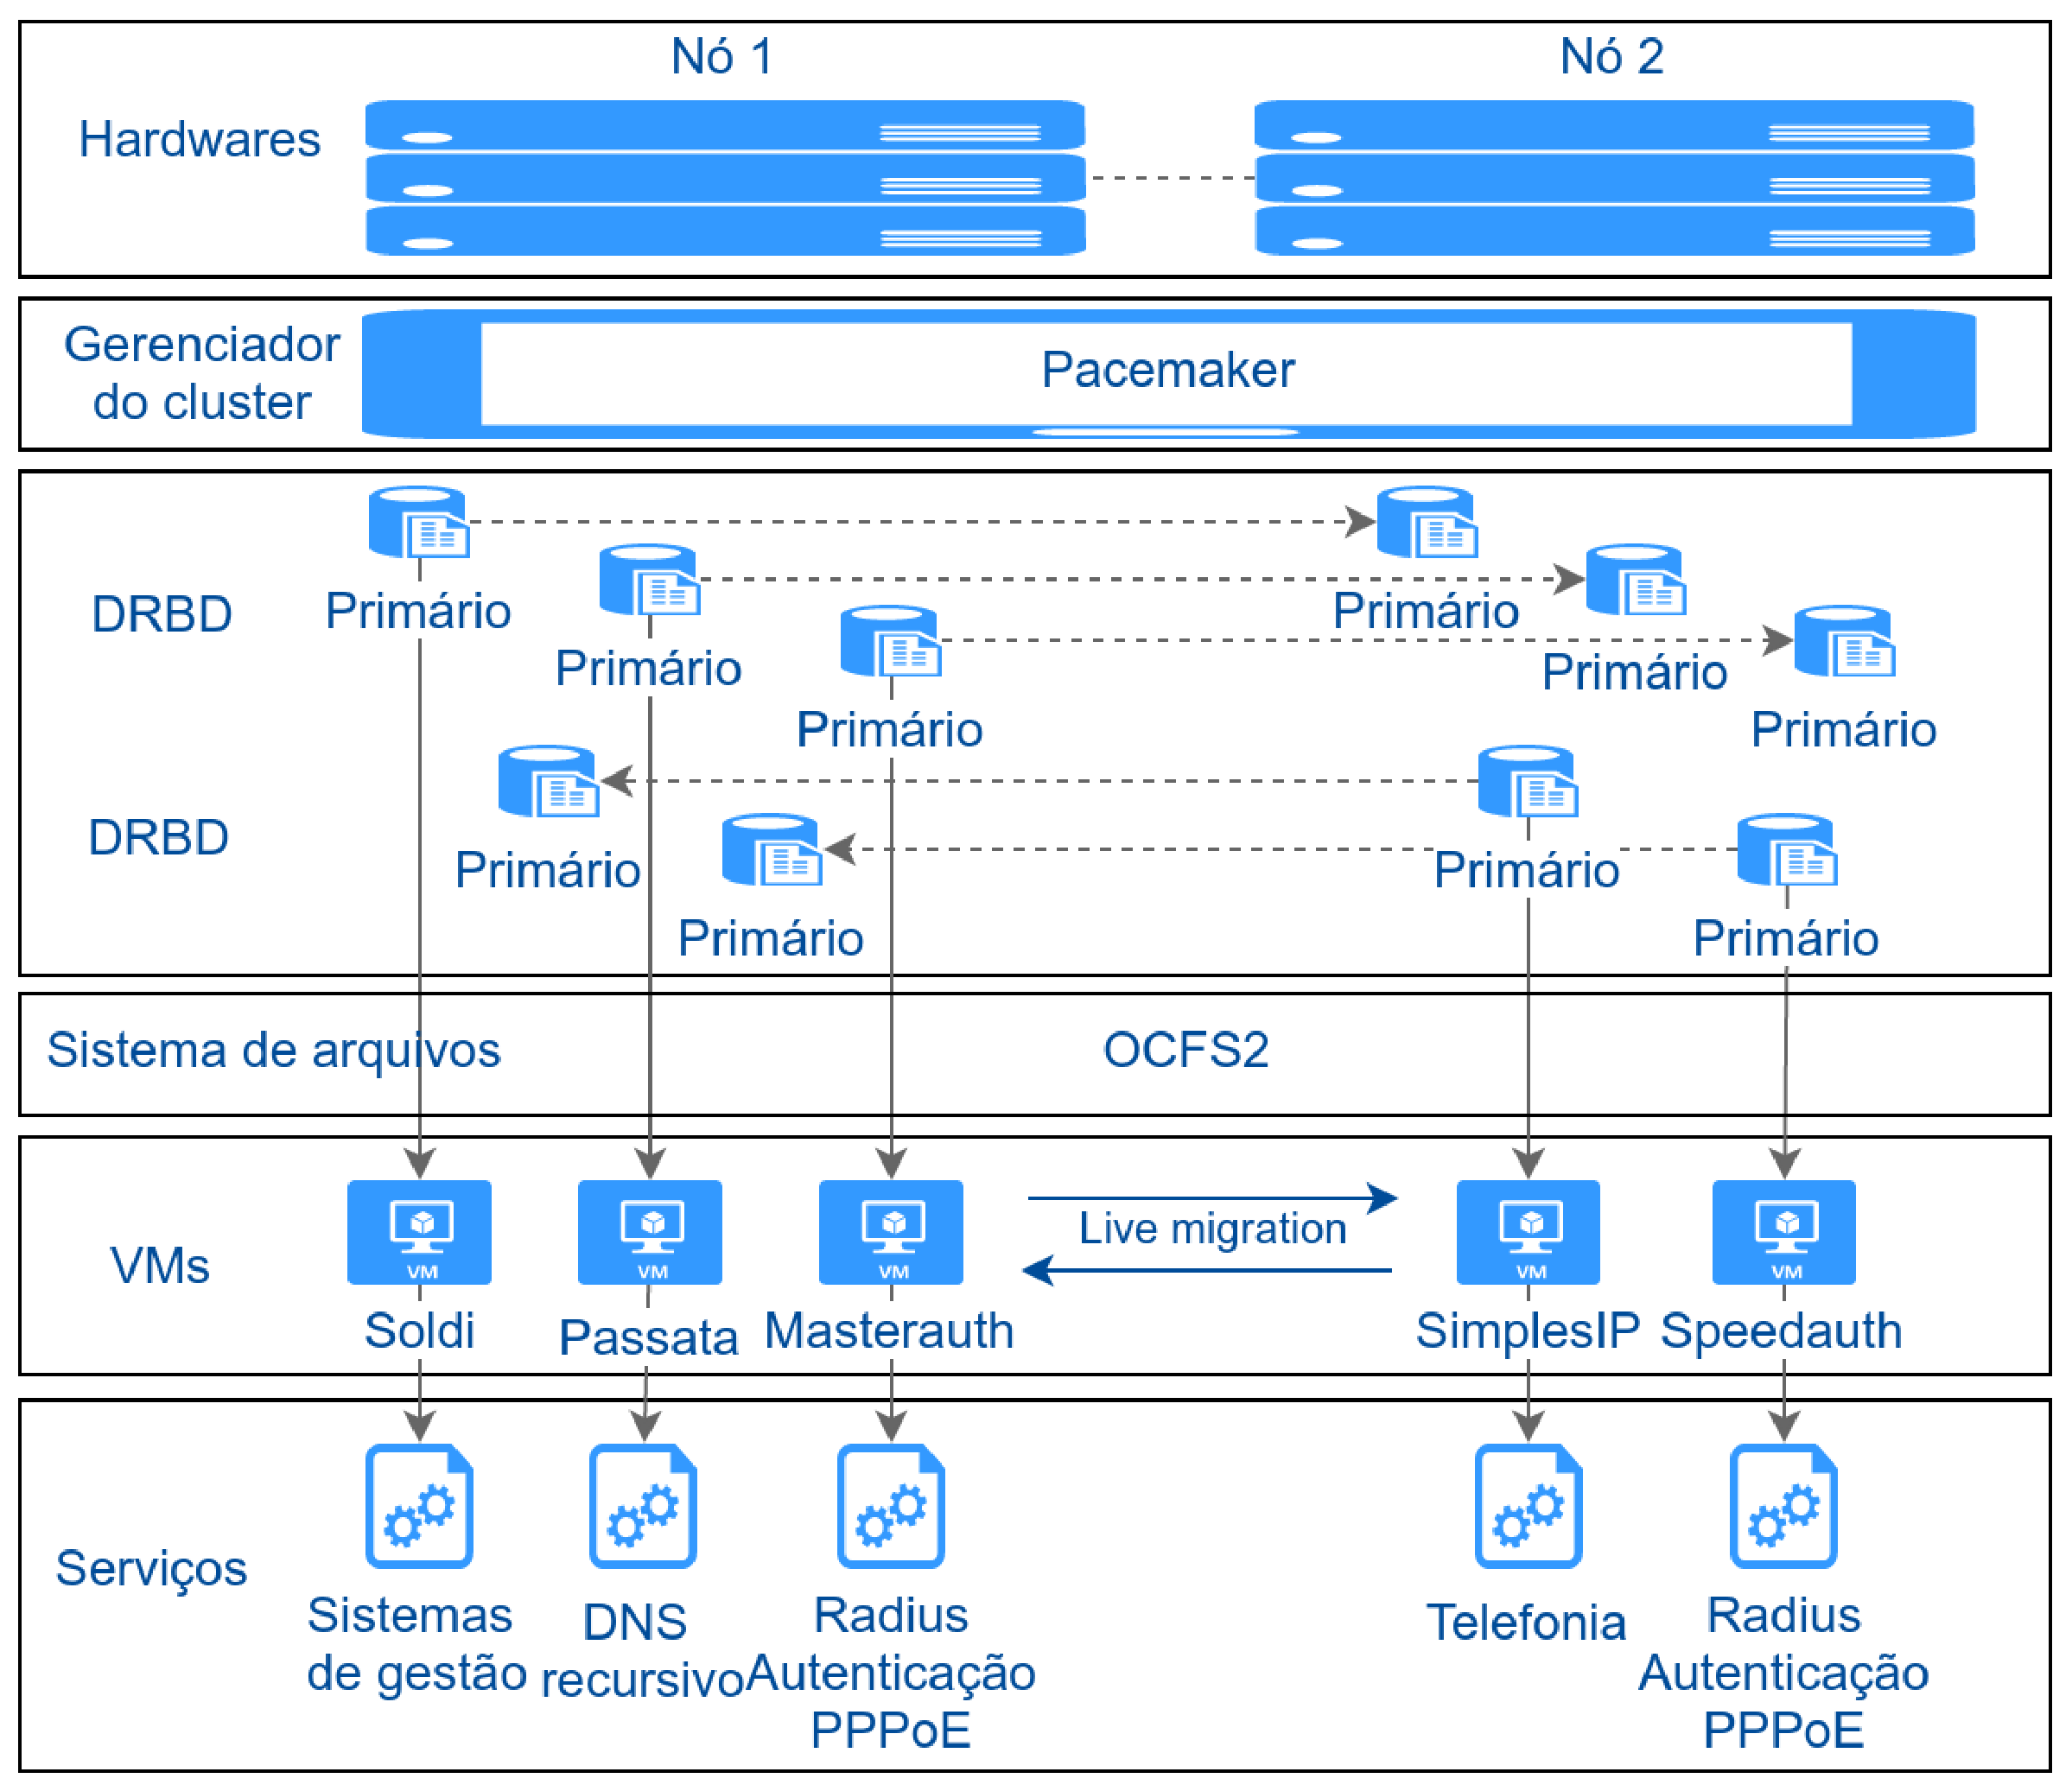
\includegraphics[width=350px]{img/projeto_estrutura.eps}
 \caption{Estrutura do \textit{cluster}.}
 \label{fig:projeto_estrutura}
\end{figure}

tabela com ips??

\section{Configuração do \ac{OS}}

Foi feita a instalação do sistema operacional \textit{Ubuntu 14.04 \ac{LTS}} nos dois servidores. A configuração feita foi a básica do sistema,
com nome do servidor, configuração de rede, localização e instalação do servidor \ac{SSH}.
Além disso, é feito as configurações padrões adotadas pela empresa, como por exemplo, ferramentas de monitoramento, atualização automática
e \textit{firewall}.

\section{Configuração de rede}

Um requisito para incluir as máquinas virtuais a uma rede é criar uma \textit{bridge}. A instalação é feita através do comando:
\begin{lstlisting}[language=bash]
  $ apt-get install bridge-utils
\end{lstlisting}

Além disso, é necessário instalar e configurar o \textit{link agregation}

\section{Configuração de disco}


\section{Configuração do ambiente virtualizado}

chaves ssh root??

\section{Configuração do cluster}

